\section{弱解}
\label{sec:cons-weak}

特征线在$T^{*}$失效，收支平衡并没有失效。路上的车不会因为斜率变成无穷而消失，式~\eqref{eq:cons-balance}依然有意义。我们需要一种不依赖导数的方式说出“解满足方程”，并回答间断会以多快的速度移动。

\subsection{积分守恒}
\label{subsec:cons-integral}

把式~\eqref{eq:cons-balance}对时间从$t_1$积分到$t_2$，得到时空矩形上的收支账：
\begin{equation}
  \begin{aligned}
    &\int_a^b u(x,t_2)\,\mathrm{d}x-\int_a^b u(x,t_1)\,\mathrm{d}x\\
    &\qquad+\int_{t_1}^{t_2}F(u(b,t))\,\mathrm{d}t
    -\int_{t_1}^{t_2}F(u(a,t))\,\mathrm{d}t=0 .
  \end{aligned}
  \label{eq:cons-box}
\end{equation}

图~\ref{fig:cons-box}把四项画在$(x,t)$平面上：矩形的上下两边记录总量，左右两边记录流过的量。把$(F(u),u)$看成$(x,t)$平面上的向量场，式~\eqref{eq:cons-box}说的是这个场穿过矩形边界的净通量为零。间断线可以从矩形中穿过，这四项仍然都有意义。

\begin{BookInlineFigure}
  \centering
  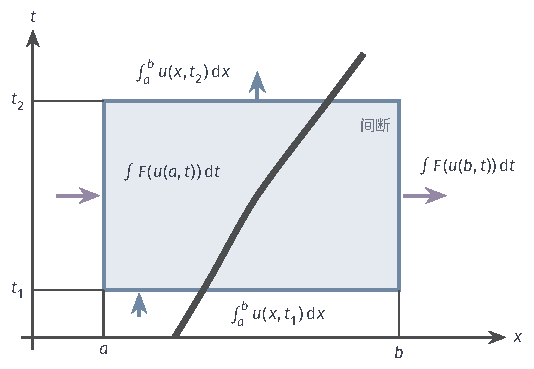
\includegraphics[width=90.4mm]{figures/06-differential-equations/02-partial-differential-equations/tikz/cons-box/figure.pdf}
  \caption{时空矩形上的收支。上下两边的蓝色箭头记录$t_2$、$t_1$时刻区间内的总量，左右两边的紫色箭头记录时段内流入、流出的量。深灰粗线是一条间断线，它穿过矩形时四项仍有定义。}
  \label{fig:cons-box}
\end{BookInlineFigure}

\paragraph{用光滑权重代替矩形}
用矩形检验有两点不便：它要用到$u$在线段上的值，而$u$只是有界可测时这样的值没有确切含义；矩形的边角也不便做微积分。办法是把矩形的示性函数换成光滑的权重$\varphi$，如图~\ref{fig:cons-test-weight}。这就像用一个边缘柔和的窗口观察收支，$\varphi$在窗口内部几乎是常数，它的导数集中在边缘附近，而边缘正是收支发生的地方。

\begin{BookInlineFigure}
  \centering
  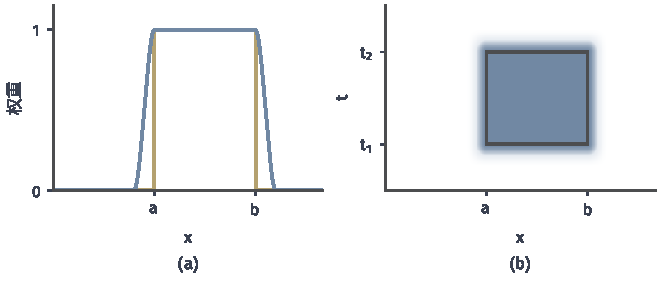
\includegraphics[width=112mm]{figures/06-differential-equations/02-partial-differential-equations/matplotlib/cons-test-weight/figure.pdf}
  \caption{用光滑权重代替矩形。(a)一维剖面：黄线是示性函数，蓝线是光滑的近似。(b)时空平面上的权重$\varphi$，颜色越深值越大，黑框是矩形$[a,b]\times[t_1,t_2]$。$\varphi$的导数只在黑框附近不为零。}
  \label{fig:cons-test-weight}
\end{BookInlineFigure}

设$u$是$C^1$解，$\varphi\in C_c^{\infty}(\mathbb{R}\times[0,\infty))$是\term{测试函数}（test function）。它在$t=0$可以不为零，在大的$\lvert x\rvert$和$t$上为零。把式~\eqref{eq:cons-law}乘以$\varphi$再积分：
\[
  \int_0^{\infty}\!\!\int_{\mathbb{R}}\bigl(\partial_tu+\partial_xF(u)\bigr)\varphi\,\mathrm{d}x\,\mathrm{d}t=0 .
\]

对$t$分部积分时，下限$t=0$留下一项$-\int_{\mathbb{R}}u_0\,\varphi(\cdot,0)\,\mathrm{d}x$；对$x$分部积分没有边界项。所有导数都转到$\varphi$上之后，得到下面的定义。

\begin{definition}[弱解]
\label{def:cons-weak-solution}
设$u_0\in L^{\infty}(\mathbb{R})$，$F\in C^1(\mathbb{R})$。有界可测函数$u$称为问题~\eqref{eq:cons-law}、\eqref{eq:cons-initial}的\term{弱解}（weak solution），若对每个$\varphi\in C_c^{\infty}(\mathbb{R}\times[0,\infty))$，
\begin{equation}
  \int_0^{\infty}\!\!\int_{\mathbb{R}}\bigl(u\,\partial_t\varphi+F(u)\,\partial_x\varphi\bigr)\,\mathrm{d}x\,\mathrm{d}t
  +\int_{\mathbb{R}}u_0\,\varphi(\cdot,0)\,\mathrm{d}x=0 .
  \label{eq:cons-weak}
\end{equation}
\end{definition}

式~\eqref{eq:cons-weak}没有$u$的导数，间断的$u$也能代入。初值的进入方式值得留意：$\varphi$在$t=0$不必为零，第二项正是下边界上的收支。若只取在$t=0$附近为零的$\varphi$，初值就看不见了。

取$\varphi$趋于矩形的示性函数，$\partial_t\varphi$在矩形上下边附近集中，$\partial_x\varphi$在左右边附近集中，式~\eqref{eq:cons-weak}的极限就回到式~\eqref{eq:cons-box}，对几乎所有的$a,b,t_1,t_2$成立。弱形式与矩形收支说的是同一件事。

弱解的概念确实推广了经典解，下面的引理说明两者在光滑情形下一致。

\begin{lemma}[经典解与弱解]
\label{lem:cons-classical-weak}
设$u\in C^1(\mathbb{R}\times[0,\infty))$有界，$F\in C^1$，$u_0$连续有界。则$u$是经典解（满足式~\eqref{eq:cons-law}、\eqref{eq:cons-initial}）当且仅当$u$满足式~\eqref{eq:cons-weak}。
\end{lemma}

\begin{proof}
必要性就是上面的分部积分。

充分性：式~\eqref{eq:cons-weak}对$u$反向分部积分。先取在$t=0$附近为零的$\varphi$，得到
\[
  \int_0^{\infty}\!\!\int_{\mathbb{R}}\bigl(\partial_tu+\partial_xF(u)\bigr)\varphi\,\mathrm{d}x\,\mathrm{d}t=0 .
\]
被积函数中的括号连续，若在某点不为零，取该点附近符号一致的$\varphi\geq0$，积分不为零，矛盾。所以式~\eqref{eq:cons-law}处处成立。

再取一般的$\varphi$，反向分部积分后内部的项已经为零，剩下
\[
  \int_{\mathbb{R}}\bigl(u_0-u(\cdot,0)\bigr)\varphi(\cdot,0)\,\mathrm{d}x=0 .
\]
$\varphi(\cdot,0)$可以是任意的$C_c^{\infty}$函数，所以$u(\cdot,0)=u_0$。
\end{proof}

\paragraph{分段满足方程并不够}
弱形式放宽了要求，但并非什么间断都行。取初值$u_0=1$（$x<0$）、$u_0=0$（$x>0$）。候选函数“间断永远不动”，即$u(x,t)=u_0(x)$，在间断线两侧都是常数，逐点满足方程。

用式~\eqref{eq:cons-box}在矩形$[-1,1]\times[0,1]$上算账，见图~\ref{fig:cons-wrong-speed}(a)。区间内的总量两个时刻都是$1$，变化量为零。左端流入$F(1)\cdot1=1/2$，右端流出$F(0)\cdot1=0$，净流入为$1/2$。账对不上，因为流进来的$1/2$没有地方去。

如果间断以速度$1/2$右移，$t=1$时总量变成$3/2$，增加的$1/2$恰好是净流入，账就平了，见图~\ref{fig:cons-wrong-speed}(b)。可见分段满足方程还不够，间断的移动速度必须与流入流出相配。下一小节给出这个条件。

\begin{BookInlineFigure}
  \centering
  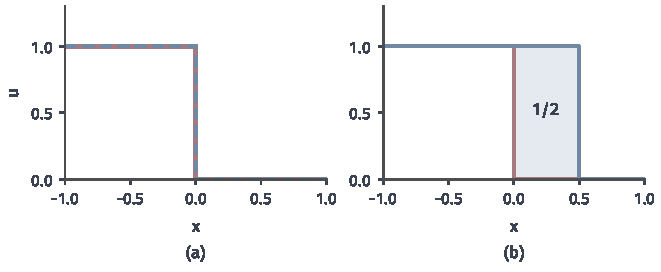
\includegraphics[width=112mm]{figures/06-differential-equations/02-partial-differential-equations/matplotlib/cons-wrong-speed/figure.pdf}
  \caption{间断速度与收支账，初值为左$1$右$0$的阶跃（红），$t=1$时的候选解为蓝线。(a)间断不动：总量不变，净流入的$1/2$无处安放。(b)间断以速度$1/2$右移：浅蓝矩形的面积$1/2$恰好等于净流入。}
  \label{fig:cons-wrong-speed}
\end{BookInlineFigure}

\paragraph{收支账选不出解}
反过来，把收支账算平也未必就够了。取Burgers方程和相反的阶跃：$u_0=0$（$x<0$）、$u_0=1$（$x>0$）。下面两个函数的初值都是这个阶跃：
\[
  u^{\mathrm{j}}(x,t)=\begin{cases}0,&x<t/2,\\1,&x>t/2,\end{cases}\qquad
  u^{\mathrm{f}}(x,t)=\begin{cases}0,&x\leq0,\\x/t,&0<x<t,\\1,&x\geq t.\end{cases}
\]

在矩形$[-2,2]\times[0,1]$上算账。初始总量是$2$，右端流出$F(1)\cdot1=1/2$，左端不流入，所以$t=1$时总量应为$3/2$。对$u^{\mathrm{j}}$，$t=1$时值为$1$的部分长度是$3/2$；对$u^{\mathrm{f}}$，总量是
\[
  \int_0^1x\,\mathrm{d}x+1\cdot1=\frac32 .
\]
两个账都平，差别只是把图~\ref{fig:cons-same-ledger}中两块面积相等的小三角形互换了位置。

\begin{BookInlineFigure}
  \centering
  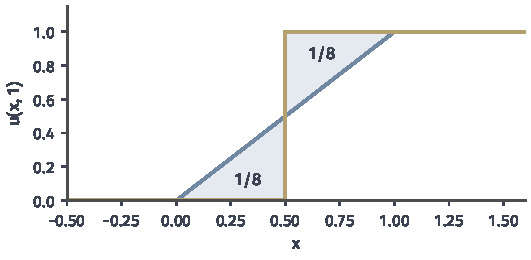
\includegraphics[width=90mm]{figures/06-differential-equations/02-partial-differential-equations/matplotlib/cons-same-ledger/figure.pdf}
  \caption{同一阶跃初值的两个候选解在$t=1$的形状：黄线是带间断的$u^{\mathrm{j}}$，蓝线是连续的$u^{\mathrm{f}}$。两块浅蓝三角形的面积都是$1/8$，一增一减，总量相同。}
  \label{fig:cons-same-ledger}
\end{BookInlineFigure}

矩形收支是必要条件，这里只验证了一个矩形。下一小节的定理会说明这两个函数确实都是弱解。经典解一定满足弱形式，但弱形式可以容许同一个初值有多个解，这是放宽解的概念要付的代价。

\subsection{跳跃条件}
\label{subsec:cons-jump}

间断以多快的速度移动？设间断两侧的状态是$u_-$（左）和$u_+$（右），间断的速度是$s$。

换到跟着间断一起运动的坐标系，见图~\ref{fig:cons-moving-jump}(b)。在这个坐标系里间断静止，所有物质的速度都减去了$s$，通量相应变成$F(u)-su$。间断是一条线，存不下任何东西，所以从左边进入的量必须等于从右边流出的量：
\[
  F(u_-)-s\,u_-=F(u_+)-s\,u_+ .
\]

\begin{BookInlineFigure}
  \centering
  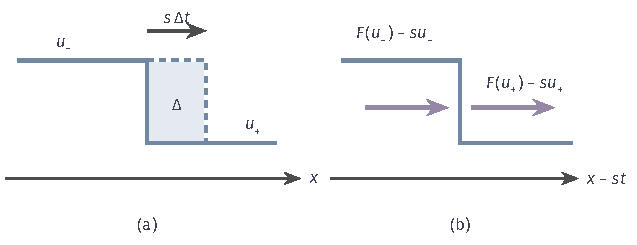
\includegraphics[width=107.9mm]{figures/06-differential-equations/02-partial-differential-equations/tikz/cons-moving-jump/figure.pdf}
  \caption{间断处的收支。(a)实验室坐标：时间$\Delta t$内间断移动$s\Delta t$，浅蓝矩形内的总量变化$(u_--u_+)s\Delta t$必须等于净流入。(b)随间断运动的坐标：相对通量$F(u)-su$在间断两侧相等，紫色箭头表示这两股流量。}
  \label{fig:cons-moving-jump}
\end{BookInlineFigure}

移项就得到\term{Rankine--Hugoniot条件}（Rankine--Hugoniot condition）。下面的定理说明，这个条件恰好刻画了分段光滑函数何时是弱解。

\begin{theorem}[Rankine--Hugoniot条件]
\label{thm:cons-rh}
设$F\in C^1$，$V\subset\mathbb{R}\times(0,\infty)$是开集，$C^1$曲线$x=\gamma(t)$把$V$分成左右两部分$V_-$、$V_+$。设$u$在$V_\pm$内是$C^1$的并满足式~\eqref{eq:cons-law}，$u$及其一阶偏导都能连续延拓到曲线的两侧，单侧极限记为$u_\pm(t)$。则$u$对所有$\varphi\in C_c^{\infty}(V)$满足
\begin{equation}
  \iint_V\bigl(u\,\partial_t\varphi+F(u)\,\partial_x\varphi\bigr)\,\mathrm{d}x\,\mathrm{d}t=0
  \label{eq:cons-rh-weak}
\end{equation}
当且仅当在曲线上
\begin{equation}
  \gamma'(t)\,\bigl(u_+-u_-\bigr)=F(u_+)-F(u_-).
  \label{eq:cons-rh}
\end{equation}
\end{theorem}

\begin{proof}
考虑$(x,t)$平面上的向量场$\bm{W}=(F(u)\varphi,\ u\varphi)$。在$V_\pm$内，利用式~\eqref{eq:cons-law}，
\[
  \nabla_{(x,t)}\cdot\bm{W}=F(u)\,\partial_x\varphi+u\,\partial_t\varphi .
\]

$\varphi$在$V$的边界附近为零，所以在$V_-$上用散度定理时，只有曲线部分有贡献。曲线$x-\gamma(t)=0$上指向$V_+$（即$V_-$的外法向）的方向是$(1,-\gamma')$，弧长元是$\sqrt{1+\gamma'^2}\,\mathrm{d}t$，单位化因子抵消，于是
\[
  \iint_{V_-}\bigl(u\,\partial_t\varphi+F(u)\,\partial_x\varphi\bigr)\,\mathrm{d}x\,\mathrm{d}t
  =\int\bigl(F(u_-)-\gamma'u_-\bigr)\,\varphi(\gamma(t),t)\,\mathrm{d}t .
\]

在$V_+$上外法向反号，得到
\[
  \iint_{V_+}\bigl(u\,\partial_t\varphi+F(u)\,\partial_x\varphi\bigr)\,\mathrm{d}x\,\mathrm{d}t
  =-\int\bigl(F(u_+)-\gamma'u_+\bigr)\,\varphi(\gamma(t),t)\,\mathrm{d}t .
\]

两式相加，积分等式等价于
\[
  \int\Bigl(F(u_-)-F(u_+)-\gamma'(u_--u_+)\Bigr)\,\varphi(\gamma(t),t)\,\mathrm{d}t=0
\]
对所有$\varphi$成立。括号里的函数连续，$\varphi$在曲线上的值可以任取，所以这等价于括号恒为零，即式~\eqref{eq:cons-rh}。
\end{proof}

定理针对$t>0$的内部。若分段$C^1$的$u$在各块上取到相应的初值，边界$t=0$的项恰好给出式~\eqref{eq:cons-weak}中的初值积分，所以$u$是弱解当且仅当每条间断线上式~\eqref{eq:cons-rh}成立。有两个特殊情形要留意。$u_+=u_-$时式~\eqref{eq:cons-rh}自动成立，所以$u$连续、仅导数间断的折线不需要额外条件，前面的$u^{\mathrm{f}}$就属于这种情形。条件的另一面是，它只约束速度，不约束两侧状态的相对大小。

\paragraph{波速是通量的弦斜率}
$u_-\neq u_+$时，式~\eqref{eq:cons-rh}给出
\begin{equation}
  s=\frac{F(u_+)-F(u_-)}{u_+-u_-},
  \label{eq:cons-shock-speed}
\end{equation}
它是通量图像上连接两个状态的弦的斜率，如图~\ref{fig:cons-rh-chord}。由积分中值定理，$s$是$F'$在$u_-$与$u_+$之间的平均值。Burgers方程的弦斜率特别简单：
\begin{equation}
  s=\frac{u_-+u_+}{2}.
  \label{eq:cons-burgers-speed}
\end{equation}
前面的阶跃取$u_-=0$、$u_+=1$，$s=1/2$，所以$u^{\mathrm{j}}$确实是弱解；$u^{\mathrm{f}}$由两条连续接缝组成，也是弱解。一个初值，两个弱解。

\begin{BookInlineFigure}
  \centering
  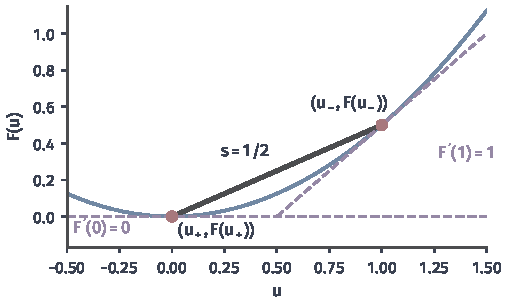
\includegraphics[width=86mm]{figures/06-differential-equations/02-partial-differential-equations/matplotlib/cons-rh-chord/figure.pdf}
  \caption{Rankine--Hugoniot速度的几何含义，$F=u^2/2$（蓝）。两个红点是状态$u_-=1$、$u_+=0$，深灰粗线是弦，斜率$s=1/2$。紫色虚线是两端的切线，斜率$F'(1)=1$与$F'(0)=0$，$s$介于两者之间。}
  \label{fig:cons-rh-chord}
\end{BookInlineFigure}

\paragraph{斜坡初值的后续}
现在可以接着算斜坡~\eqref{eq:cons-ramp}。$t=1$时解变成左$1$右$0$的台阶，位置在$x=1$。此后沿用这个台阶，令间断从$(1,1)$出发，由式~\eqref{eq:cons-burgers-speed}，速度是$1/2$，于是间断线为$x=(1+t)/2$，解为
\begin{equation}
  u(x,t)=\begin{cases}1,&x<(1+t)/2,\\0,&x>(1+t)/2,\end{cases}\qquad t\geq1.
  \label{eq:cons-ramp-shock}
\end{equation}

图~\ref{fig:cons-ramp-shock}(a)中，左侧的特征线以速度$1$从后面追上间断，右侧的特征线停在原地等间断到来，都终止在间断线上。

\begin{BookInlineFigure}
  \centering
  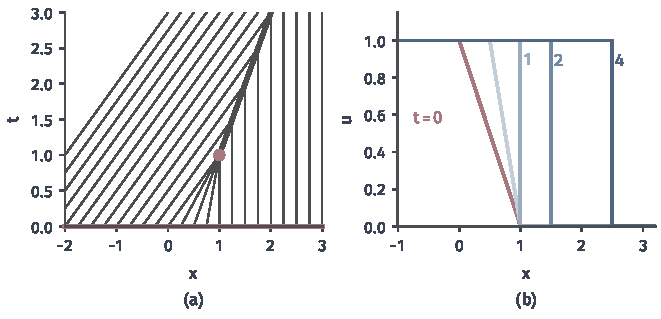
\includegraphics[width=112mm]{figures/06-differential-equations/02-partial-differential-equations/matplotlib/cons-ramp-shock/figure.pdf}
  \caption{斜坡初值的解。(a)特征线（细线）在红点$(1,1)$汇聚，此后深灰粗线$x=(1+t)/2$是间断线，两侧的特征线都在它上面终止。(b)红线是$t=0$，蓝色由浅到深是$t=0.5,1,2,4$。}
  \label{fig:cons-ramp-shock}
\end{BookInlineFigure}

\paragraph{等面积法则}
式~\eqref{eq:cons-ramp-shock}还可以换一个角度得到。沿特征线得到的多值图像虽然不是函数，但曲线下的面积是守恒的。把图像写成参数形式$(x_0+tu_0(x_0),\,u_0(x_0))$，带符号的面积随时间的变化是
\[
  \frac{\mathrm{d}}{\mathrm{d}t}\int u_0\,\bigl(1+t\,u_0'\bigr)\,\mathrm{d}x_0
  =\int u_0\,u_0'\,\mathrm{d}x_0=\Bigl[\frac{u_0^2}{2}\Bigr]_{-\infty}^{\infty},
\]
在初值的两端取相同的极限时为零。要把多值图像截成单值函数并保持总量，就应竖直切一刀，使切掉的两块面积相等，这称为\term{等面积法则}（equal-area rule）。

图~\ref{fig:cons-equal-area}(a)在$t=2$验证这一点。斜坡的多值图像中间一段是从$(1,0)$到$(2,1)$的线段$u=x-1$。在$x=c$处切开，左边多出的三角形面积是$(c-1)^2/2$，右边少掉的三角形面积是$(2-c)^2/2$。令两者相等，得$c=3/2$，与$x=(1+t)/2$在$t=2$的值一致。

\begin{BookInlineFigure}
  \centering
  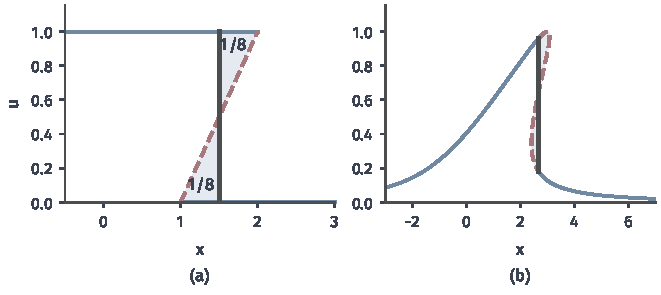
\includegraphics[width=112mm]{figures/06-differential-equations/02-partial-differential-equations/matplotlib/cons-equal-area/figure.pdf}
  \caption{等面积法则。蓝线是单值的解，红色虚线是沿特征线得到的翻转部分，深灰竖线是间断位置，两块浅蓝区域面积相等。(a)斜坡初值在$t=2$，间断位于$x=3/2$，每块面积$1/8$。(b)初值~\eqref{eq:cons-bump}在$t=3$，间断位置由数值积分得到。}
  \label{fig:cons-equal-area}
\end{BookInlineFigure}

贯穿例子~\eqref{eq:cons-bump}的间断路径没有闭式，但可以把上面两条结合起来计算。设$\gamma(t)$是间断位置，$u_\pm$是多值图像在$x=\gamma(t)$处最靠左和最靠右的分支的值，由式~\eqref{eq:cons-burgers-speed}，
\begin{equation}
  \gamma'(t)=\frac{u_-(t)+u_+(t)}{2},\qquad \gamma(T^{*})=\sqrt{3}.
  \label{eq:cons-bump-shock}
\end{equation}

这是一个常微分方程，右端要在每一步解两次特征线方程。数值积分得$\gamma(3)\approx2.677$。图~\ref{fig:cons-bump-shock}(a)中间断从红点长出，特征线不断汇入。(b)显示了波形的演化：间断形成后，峰逐渐被削低，波形的前沿始终保持一个台阶。

\begin{BookInlineFigure}
  \centering
  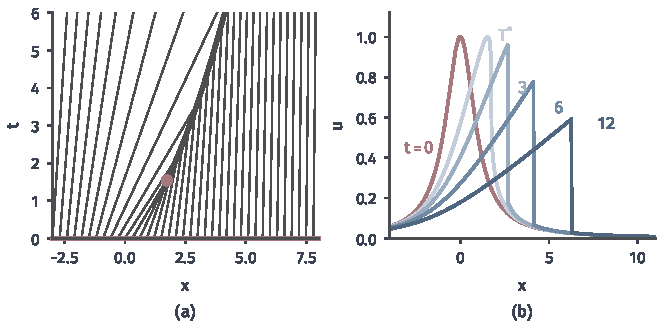
\includegraphics[width=112mm]{figures/06-differential-equations/02-partial-differential-equations/matplotlib/cons-bump-shock/figure.pdf}
  \caption{初值~\eqref{eq:cons-bump}的激波形成之后。(a)细线是特征线，它们都在深灰粗线（数值求解式~\eqref{eq:cons-bump-shock}得到的间断路径）上终止，红点是最早的相交点。(b)红线是$t=0$，蓝色由浅到深是$t=T^{*},3,6,12$，台阶越来越矮。}
  \label{fig:cons-bump-shock}
\end{BookInlineFigure}

\paragraph{同一方程的不同守恒形式}
跳跃条件依赖于哪个量守恒。$C^1$时，Burgers方程乘以$u$，得到同样成立的
\[
  \partial_t\Bigl(\frac{u^2}{2}\Bigr)+\partial_x\Bigl(\frac{u^3}{3}\Bigr)=0 .
\]
两个方程的光滑解完全相同，但把后者看作守恒律时，守恒量是$u^2/2$，通量是$u^3/3$。

对同一组状态$u_-=1$、$u_+=0$，由式~\eqref{eq:cons-shock-speed}，两种写法给出的速度分别是
\[
  s=\frac{1/2-0}{1-0}=\frac12,\qquad
  s=\frac{1/3-0}{1/2-0}=\frac23 .
\]

图~\ref{fig:cons-form-speed}画出这两条路径。所以方程写成哪一种守恒形式不是记号问题，而是在说明哪个量真正守恒；$u\,\partial_xu$这样的非守恒写法在间断处没有定义，也就无从决定速度。

\begin{BookInlineFigure}
  \centering
  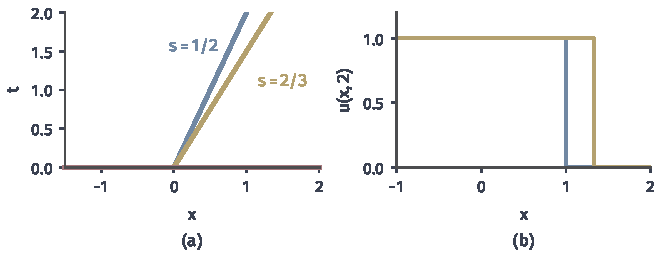
\includegraphics[width=112mm]{figures/06-differential-equations/02-partial-differential-equations/matplotlib/cons-form-speed/figure.pdf}
  \caption{守恒形式决定间断速度，状态$u_-=1$、$u_+=0$。(a)蓝线是以$u$为守恒量得到的路径$s=1/2$，黄线是以$u^2/2$为守恒量得到的路径$s=2/3$。(b)两种情形在$t=2$的形状。}
  \label{fig:cons-form-speed}
\end{BookInlineFigure}

跳跃条件只保证穿过间断的总量收支平衡。$u^{\mathrm{j}}$满足它，$u^{\mathrm{f}}$也满足，所以还要有别的办法检验传播方向是否合理。
